\documentclass[11pt,a4paper]{article}
\usepackage[margin=2.4cm]{geometry}
\usepackage[T1]{fontenc}
\usepackage{lmodern}
\usepackage{microtype}
\usepackage{graphicx}
\usepackage{booktabs,array,tabularx}
\usepackage{float}
\usepackage{caption}
\usepackage{xcolor}
\usepackage{enumitem}
\usepackage{amsmath}
\usepackage{fancyhdr}
\usepackage[round,authoryear]{natbib}
\usepackage[colorlinks=true,linkcolor=blue!50!black,citecolor=blue!50!black,urlcolor=blue!50!black]{hyperref}
\captionsetup{font=small,labelfont=bf,skip=4pt}
\setlist{nosep,leftmargin=1.4em}
\setlength{\parskip}{4pt}\setlength{\parindent}{0pt}
\newcommand{\shot}[2][0.97]{\fcolorbox{black!25}{white}{\includegraphics[width=#1\linewidth]{#2}}}
\newcommand{\RFG}{\textsc{RFG}}
\pagestyle{fancy}\fancyhf{}
\fancyhead[L]{\small Ready-to-Functional Gap on Real Kubernetes}
\fancyhead[R]{\small Pilot study}
\fancyfoot[C]{\thepage}
\renewcommand{\headrulewidth}{0.3pt}

\title{\textbf{Measuring the Ready-to-Functional Gap in Kubernetes:\\ A Fault-Injection Pilot Study on a Multi-Node Cluster}}
\author{Vinod Ravindu Perera\thanks{Correspondence: \texttt{bamunugevinod.ravinduperera@study.beds.ac.uk}}\\[2pt]
{\small Sri Lanka Institute of Information Technology (SLIIT), Malabe, Sri Lanka}\\{\small Nebula Institute of Technology, Welisara, Sri Lanka}}
\date{9 November 2026\\[2pt]\small Pilot study: five runs per condition, descriptive statistics only}

\begin{document}
\maketitle

\begin{abstract}
Kubernetes marks a Pod \emph{Ready} when its readiness probe succeeds, and a Service then routes traffic to it. A Pod can be Ready while the application inside cannot yet answer correctly. I call the time spent in this state the \emph{Ready-to-Functional Gap} (RFG). I measured it on a real three-node Kubernetes cluster (kind v0.25.0, Kubernetes 1.31) by injecting four faults (application degradation, Pod replacement, dependency restart, and Pod replacement during a dependency restart) under three readiness configurations (a shallow probe, a deep probe that checks a dependency, and a shallow probe with a passive external observer), five runs each, 60 runs in total. A ground-truth request stream sent directly to each Pod defined when the application was truly functional, and a second stream through the Service measured what users saw. An independent validator recomputed every run from raw files; 59 of 60 runs passed and one was flagged and kept. With the shallow probe, Pods stayed Ready while failing for a median of 3.6\,s (application degradation) up to 16\,s (replacement during dependency restart, two replicas summed). The failures were HTTP~200 replies with wrong content, which status-code monitoring would not flag. The deep probe had the lowest Ready-but-invalid time in every scenario but, when the shared dependency restarted, removed both replicas from the Service (median 5.9\,s without a ready Pod) and failed static pages that did not need the dependency. A passive observer detected loss in 0.05--0.15\,s with no false ``functional'' declaration in 30 observations and without altering readiness. A local simulation I built earlier predicted no gap for plain Pod replacement; on the real cluster 9 of 10 shallow-probe runs showed a small positive gap (0.08--0.62\,s). The results are directional, not conclusive: sample sizes are small, the setting is one laptop, and the sign of one simulated effect did not carry over.
\end{abstract}

\noindent\textbf{Keywords:} Kubernetes, readiness probes, gray failure, fault injection, service availability, observability.

%--------------------------------------------------------------------
\section{Introduction}
Kubernetes decides whether a Pod should receive Service traffic from its readiness state: a Pod whose readiness probe fails is removed from the matching Service endpoints \citep{k8sprobes}, and an endpoint's \emph{ready} condition is derived from the Pod's Ready condition \citep{k8sendpointslices}. The probe is an application-defined check, so the platform can only be as accurate as that check. If the probe passes while the application cannot yet serve correct answers, the Service keeps sending real users to a Pod that is wrong.

I call the interval between a Pod being Ready and the application being functionally valid the \textbf{Ready-to-Functional Gap (RFG)} (Figure~\ref{fig:concept}). The question is practical: how long is this window on a real cluster, what do users see inside it, and what does it cost to close it?

\begin{figure}[H]
\centering\shot[0.8]{figures/R01-concept-diagram.png}
\caption{The Ready-to-Functional Gap. The Pod turns Ready (left dashed line) before the application works (right dashed line); users receive wrong or failed answers in between.}
\label{fig:concept}
\end{figure}

\paragraph{Research questions.}
\begin{description}[style=nextline]
\item[RQ1] Does the gap occur under real Kubernetes behaviour, and how long is it?
\item[RQ2] Are users, reaching the application through a Service, exposed to it?
\item[RQ3] Does a deep readiness probe reduce functional failures, and does it cause unnecessary endpoint withdrawal?
\item[RQ4] Can a standalone observer detect loss of functionality and recovery without changing Pod readiness?
\item[RQ5] How much do EndpointSlice updates add to the measured gap?
\end{description}

\paragraph{Contributions.} (i) A measurement design that defines ``functional'' from a ground-truth stream independent of the readiness mechanism; (ii) 60 fault-injection runs on a real multi-node cluster, each recomputed by an independent validator; (iii) a comparison of a shallow probe, a deep probe and a passive observer; and (iv) a side-by-side comparison with my earlier local simulation, including one result that did not reproduce.

\paragraph{Scope.} This is a pilot. I report medians and ranges of five runs per condition and make no significance claims. I did not conduct a systematic literature review for this paper; the only external sources cited are the Kubernetes documentation pages on which the definitions above rest. A literature review is listed under future work.

%--------------------------------------------------------------------
\section{Method}
\subsection{Environment}
All runs used a single Windows~11 laptop (12 CPUs, about 15\,GB RAM) with WSL~2 and Docker Desktop. The cluster was created with kind v0.25.0 \citep{kindsite}, node image Kubernetes v1.31.2, one control-plane node and two workers; the \texttt{kubectl} client was v1.37.2. Figure~\ref{fig:env} shows the environment check and cluster creation (the full command-line record is in Appendix~\ref{app:evidence}). The whole 60-run pilot finished in under 30 minutes.

\begin{figure}[H]
\centering
\shot[0.78]{figures/S02-diagnose-environment.png}\\[4pt]
\shot[0.78]{figures/S05-create-cluster.png}
\caption{Top: environment diagnostic (Docker client and server, 12 CPUs, about 15\,GB RAM). Bottom: creation of the three-node cluster \texttt{rfg}, Ready after 12\,s.}
\label{fig:env}
\end{figure}

\subsection{System under test}
Two application replicas (\texttt{r0.1}, \texttt{r1.1}) run behind a ClusterIP Service. Each depends on one data store deployed as a StatefulSet with a persistent volume; after a restart the store answers ``still loading'' while it replays its write-ahead log. The application serves a transaction endpoint, which needs the store, and a static endpoint, which does not. In degraded mode the application keeps answering \texttt{HTTP 200} but returns a fallback payload, so a status-code check cannot tell the two apart. Kubelet probes use a 1\,s period, 1\,s timeout and failure threshold~3; no liveness or startup probes are configured. The application and its business logic are the unchanged code from my earlier local simulation; only addressing flags were added.

\subsection{Arms (readiness configurations)}
\begin{description}[style=nextline]
\item[A, shallow] The readiness probe succeeds if the application process answers.
\item[B, deep] The probe also pings the dependency and requires a warm cache.
\item[C, shallow + observer] Same probe as A, plus a standalone observer (5\,Hz, declares a state after 5 consecutive samples) that only records and never changes readiness.
\end{description}
Arms A and C use the same readiness probe; their differences therefore estimate run-to-run noise (Section~\ref{sec:noise}).

\subsection{Faults}
\begin{table}[H]
\centering\small
\begin{tabularx}{\linewidth}{@{}l X l@{}}
\toprule
Scenario & Fault injected & Affected replicas\\
\midrule
app-degrade & Application on \texttt{r0.1} switched to degraded (fallback) mode, then recovered & \texttt{r0.1}\\
pod-replace & Pod \texttt{r0.2} deleted with grace period 0 & replacement Pod\\
dep-restart & Store Pod deleted (log replay on restart) & \texttt{r0.1}, \texttt{r1.1}\\
replace-during-dep & Store Pod and an application Pod deleted together & replacement Pod, \texttt{r1.1}\\
\bottomrule
\end{tabularx}
\caption{The four injected faults. Each of 4 scenarios $\times$ 3 arms was repeated 5 times (60 runs).}
\label{tab:faults}
\end{table}

\subsection{Measurement}
An in-cluster collector uses a single monotonic clock, injects faults through the Kubernetes API, watches Pods and EndpointSlices, and sends four request streams:
\begin{itemize}
\item \textbf{G} (ground truth): directly to each Pod IP at 20\,Hz;
\item \textbf{U} (users): through the Service, transactions at 20\,Hz and static content at 10\,Hz;
\item \textbf{D}: a dependency ping at 10\,Hz;
\item \textbf{observer} (arm C only): 5\,Hz, detection only.
\end{itemize}
A reply is \emph{valid} if its content is correct, not merely if the status is 200.

\paragraph{Definitions.} $T_{\mathrm{func}}$ is the start of the first sustained window on stream~G (at least 20 consecutive valid samples spanning at least 1\,s). Then
\[
\mathrm{RFG}_{\mathrm{observe}} = T_{\mathrm{func}} - T_{\mathrm{Pod\,Ready}},\qquad
\mathrm{RFG}_{\mathrm{endpoint}} = T_{\mathrm{func}} - T_{\mathrm{endpoint\,available}},
\]
where a positive value means Ready before functional. \emph{Ready-but-invalid time} sums, over affected replicas, the time G was invalid while the Pod counted as Ready; \emph{false-NotReady time} sums the time G was valid while the Pod was NotReady. Because both are totals over replicas, two-replica scenarios are not directly comparable to one-replica ones. \emph{User error time} is the duration of failed or invalid replies on stream~U; \emph{zero-endpoint time} is the time the Service had no ready endpoint. Watch timestamps are receipt times at the collector, and the Pod condition's \texttt{lastTransitionTime} has only 1\,s resolution.

\subsection{Validation and data safeguards}
Before the pilot, the run script was made to refuse to overwrite existing results (Appendix Figure~\ref{fig:s07}). After every run, a separate validator recomputed the key quantities from the raw CSV files and compared them with the collector's summary, with 31--36 checks per run (file presence, sampling gaps against the expected interval, distinct replacement Pods, no invalid samples between steady state and fault, and recomputed onset and $T_{\mathrm{func}}$ values). Figure~\ref{fig:timeline} shows the validator output and event timeline of one manual test run (a Pod replaced during a dependency restart; not pilot data). In it, the replacement Pod was marked Ready at $+2.58$\,s after the fault, while sustained correct answers began at $+6.01$\,s, about 3.4\,s later.

\begin{figure}[H]
\centering\shot[0.8]{figures/S08-validator-and-timeline.png}
\caption{Validator output and event timeline of a manual test run. Times are seconds after the fault; watch events are receipt times.}
\label{fig:timeline}
\end{figure}

I did not change the validator after seeing results. The 10\,s probe-period sweep was not run.

%--------------------------------------------------------------------
\section{Results}
All 60 pilot runs completed (Figure~\ref{fig:pilot}); 59 passed validation and one was flagged (Section~\ref{sec:invalid}). All 60 are included in every statistic below. The 12 aggregate cells were additionally recomputed from the 60 per-run summary files with a separate script (0 mismatches). Values are medians [min--max] of five runs unless stated.

\begin{figure}[H]
\centering
\shot[0.8]{figures/S10-pilot-finished-60-runs.png}\\[4pt]
\shot[0.8]{figures/S11-validation-59-valid-1-invalid.png}
\caption{Top: the pilot finished with 60 runs and no runner error. Bottom: validation of the 60 run folders (59 VALID, 1 INVALID).}
\label{fig:pilot}
\end{figure}

\begin{table}[H]
\centering\footnotesize
\setlength{\tabcolsep}{3.5pt}
\begin{tabular}{@{}llcccc@{}}
\toprule
Scenario & Arm & Ready-but-invalid (s) & User error time (s) & Invalid replies & False NotReady (s)\\
\midrule
app-degrade & A & 3.65 [3.35--3.95] & 3.60 [3.05--3.80] & 39 & 0.00\\
 & B & 2.85 [2.35--3.00] & 2.75 [2.30--3.00] & 28 & 0.45\\
 & C & 3.55 [3.35--4.25] & 3.45 [3.15--4.05] & 38 & 0.00\\
\addlinespace
pod-replace & A & 0.30 [0.00--0.50] & 0.10 [0.00--0.20] & 2 & 0.00\\
 & B & 0.00 [0.00--0.00] & 0.00 [0.00--0.00] & 0 & 0.35\\
 & C & 0.35 [0.05--0.60] & 0.05 [0.00--0.40] & 1 & 0.00\\
\addlinespace
dep-restart & A & 7.65 [3.10--15.75] & 3.85 [1.55--7.84] & 75 & 0.00\\
 & B & 5.60 [3.25--5.65] & 9.10 [1.65--17.42] & 59 & 1.90\\
 & C & 5.75 [3.15--8.25] & 3.75 [1.55--4.10] & 58 & 0.00\\
\addlinespace
replace-during-dep & A & 15.95 [15.75--32.20] & 8.60 [0.05--10.25] & 163 & 0.00\\
 & B & 2.75 [2.10--2.80] & 3.96 [1.95--7.03] & 55 & 0.80\\
 & C & 8.00 [7.45--15.50] & 4.60 [4.05--9.20] & 83 & 0.00\\
\bottomrule
\end{tabular}
\caption{Main outcomes by scenario and arm (median [min--max] of 5 runs; invalid replies and false NotReady are medians). Ready-but-invalid and false-NotReady times are summed over affected replicas. Source: \texttt{aggregate.md} of the pilot.}
\label{tab:main}
\end{table}

\subsection{RQ1: the gap occurs, and it varies widely}
With the shallow probe (arms A and C), Pods stayed Ready while the ground-truth stream was invalid in every scenario involving a fault in the application or its dependency (Table~\ref{tab:main}, Figure~\ref{fig:ready}).
\begin{itemize}
\item \textbf{app-degrade:} the Pod never went NotReady and no endpoint was withdrawn, yet valid transactions failed for a median 3.65\,s (A) and 3.55\,s (C). This is gray failure by construction: the application answers HTTP~200 with a fallback payload.
\item \textbf{dep-restart:} 7.65\,s (A) and 5.75\,s (C), summed over two replicas.
\item \textbf{replace-during-dep:} the replacement Pod was reported Ready before it was functional in 10 of 10 shallow-probe runs. $\mathrm{RFG}_{\mathrm{observe}}$ values were 16.39, 8.13, 8.06, 7.97, 8.60 (A) and 3.89, 3.77, 4.70, 4.03, 7.86\,s (C); pooled median 7.9\,s (range 3.77--16.39).
\item \textbf{pod-replace} (healthy dependency): a small positive gap of 0.08--0.62\,s in 9 of 10 runs; in the tenth the replacement was functional from its first sample, so there was no degraded window to measure.
\end{itemize}

\begin{figure}[H]
\centering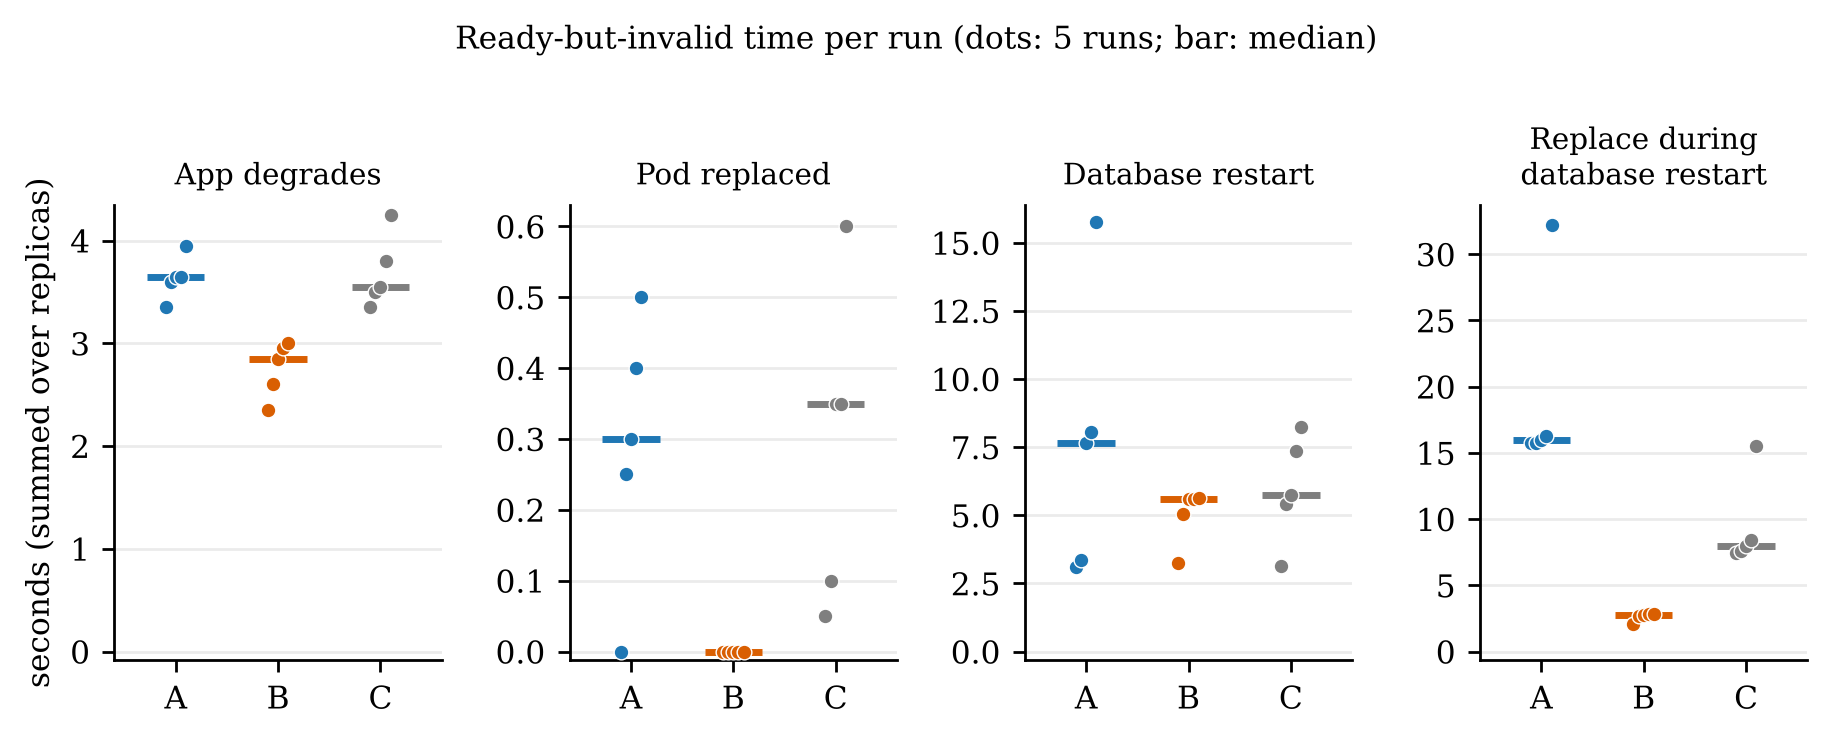
\includegraphics[width=\linewidth]{figures/fig-ready-nonfunctional.png}
\caption{Ready-but-invalid time per run for the three arms (dots: individual runs; bar: median). Arms A and C use the same probe, yet differ by about 8\,s in the last panel.}
\label{fig:ready}
\end{figure}

\subsection{RQ2: users are exposed through the Service}
Because the shallow probe kept the faulty Pods Ready (zero-endpoint time 0\,s), the Service kept routing to them. User error time through the Service was a median 3.60\,s (app-degrade A), 3.85\,s (dep-restart A) and 8.60\,s (replace-during-dep A), with 39, 75 and 163 invalid replies. The invalid replies are HTTP~200 responses with wrong content. In dep-restart, the shallow arms had a median of 75 (A) and 58 (C) invalid replies but at most one HTTP error per run (Section~\ref{sec:http}), so status-code alerting would show little. Plain Pod replacement mostly protected users (median 0.10\,s for A, 0.05\,s for C). A plausible reason is that the Service stops routing to a deleted Pod quickly; I did not isolate this.

\begin{figure}[H]
\centering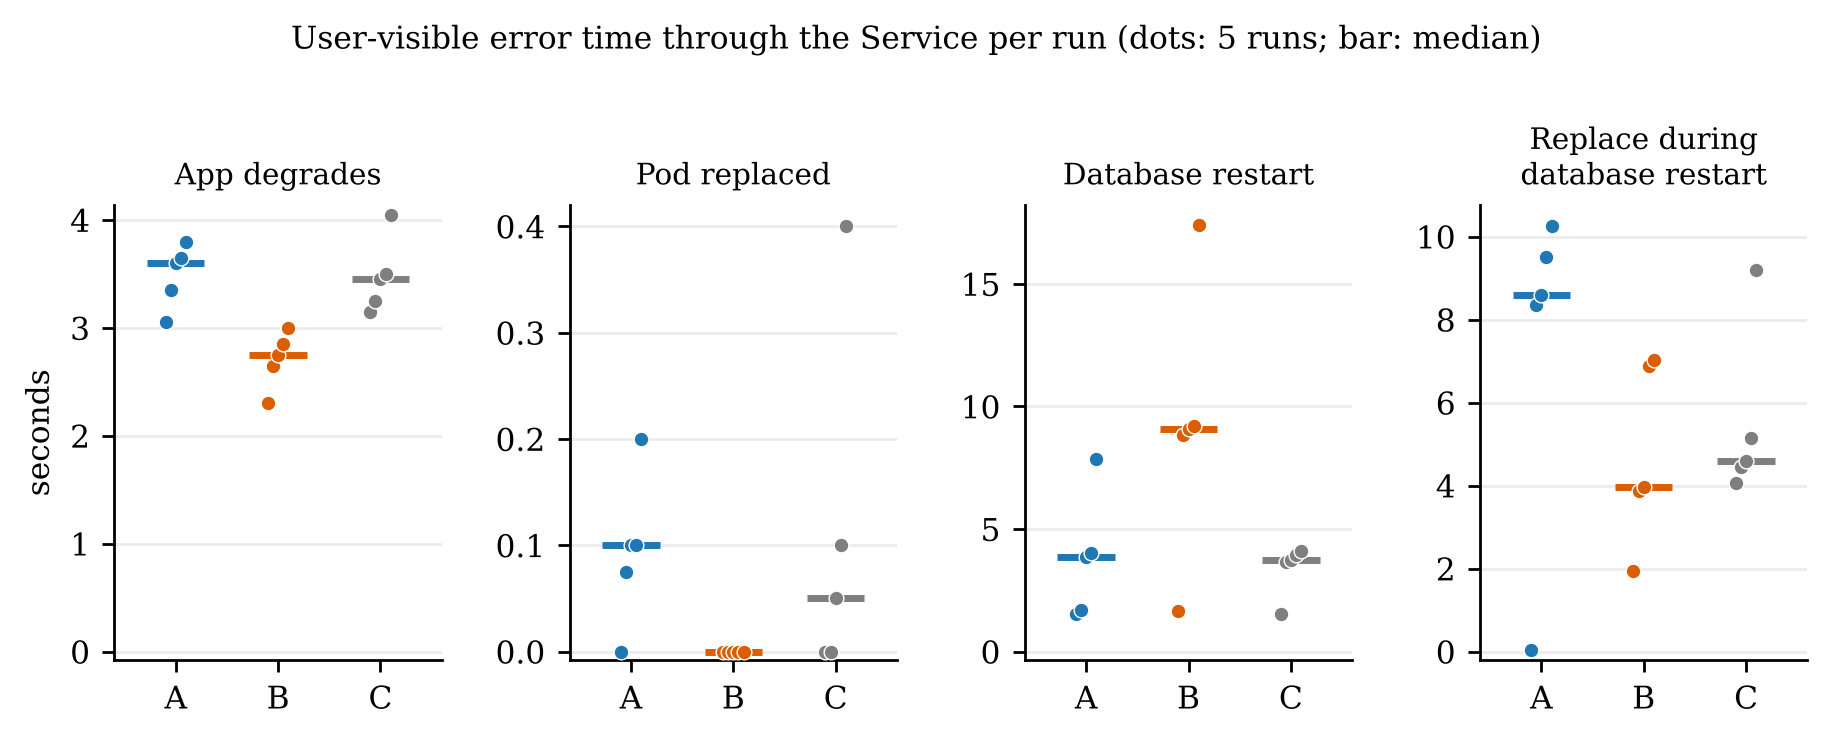
\includegraphics[width=\linewidth]{figures/fig-user-error.png}
\caption{User-visible error time through the Service, per run.}
\label{fig:user}
\end{figure}

\subsection{RQ3: the deep probe helps, and it costs endpoints}\label{sec:rq3}
\paragraph{Benefit.} Ready-but-invalid time was lowest for the deep probe (arm~B) in all four scenarios; in replace-during-dep its median was 2.75\,s against 15.95\,s (A) and 8.00\,s (C). Relative to the pooled shallow runs (A and C combined), the B-to-shallow median ratios were 0.79 (app-degrade), 0.85 (dep-restart) and 0.18 (replace-during-dep); in pod-replace all five B runs were exactly 0. With arm~B the replacement Pod became Ready only after it was functional: $\mathrm{RFG}_{\mathrm{observe}}$ medians were $-0.44$, $-0.92$, $-0.32$ and $-0.25$\,s.

\paragraph{Cost.} In dep-restart both replicas depend on the same store, so the deep probe withdrew both. Median zero-endpoint time was 5.90\,s (range 0--13.96; positive in 4 of 5 runs, Figure~\ref{fig:zero}), and static content, which does not need the store, failed for a median of 6.23\,s (0--13.45). User error time was 9.10\,s [1.65--17.42] against 3.85\,s (A) and 3.75\,s (C); four of the five arm-B runs (8.83--17.42\,s) exceeded the largest shallow-arm value in that scenario (7.84\,s). Pods also stayed NotReady after they recovered (false-NotReady medians 0.45, 0.35, 1.90 and 0.80\,s, against 0.00\,s for arms A and C, whose largest single value was 0.05\,s), and the probes made a median of 21.5 dependency calls per run (range 17--26) while arms A and C made none.

\begin{figure}[H]
\centering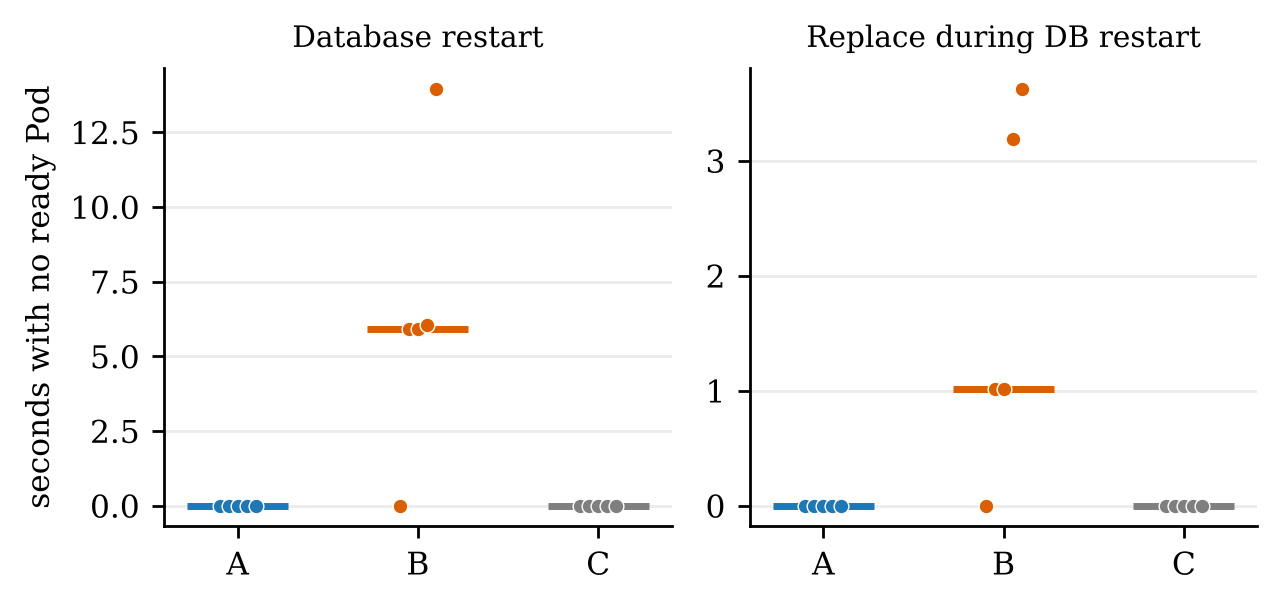
\includegraphics[width=0.72\linewidth]{figures/fig-zero-endpoint.png}
\caption{Time with no ready Pod behind the Service (zero-endpoint time), per run. Only the deep probe (B) produced non-zero values.}
\label{fig:zero}
\end{figure}

The trade-off depends on the scenario: in replace-during-dep the deep probe had less user error time than A (3.96\,s vs 8.60\,s) but also 1.02\,s of zero endpoints. Differences between arms of a few seconds should be read with the noise estimate below in mind.

\subsection{RQ4: a passive observer detects the gap}
\begin{table}[H]
\centering\small
\begin{tabular}{@{}lcccc@{}}
\toprule
Scenario & Observations & Loss detected after onset (s) & Recovery declared & False ``functional''\\
\midrule
app-degrade & 5 & 0.052 [0.051--0.151] ($n{=}5$) & 5 & 0\\
dep-restart & 10 & 0.052 [$-$0.001--0.102] ($n{=}10$) & 10 & 0\\
pod-replace & 5 & not defined & 5 & 0\\
replace-during-dep & 10 & 0.151 [0.002--0.152] ($n{=}5$ of 10) & 10 & 0\\
\bottomrule
\end{tabular}
\caption{Observer performance in arm C (median [min--max]). Loss detection time is undefined for pod-replace and was defined for 5 of 10 observations in replace-during-dep; I did not examine why.}
\label{tab:observer}
\end{table}
The observer declared recovery in all 30 observations and made no premature declaration (0 of 30). It never changed readiness: arm-C false-NotReady and zero-endpoint times were 0\,s in every scenario, as for arm~A. The cost was about 139 extra requests per run (range 107--197). Its recovery confirmation preceded the ground-truth reference by a median 0.10--0.20\,s; since the reference sample completes a longer window (20 samples over 1\,s) than the observer's confirmation (5 samples), a small negative value is expected and does not mean the observer predicts recovery. The observer samples at 5\,Hz, so its resolution is about 0.2\,s. This is detection, not a mitigation; what to do with the signal was not tested.

\subsection{RQ5: EndpointSlices add little}
In the eight cells where a Ready transition occurred, the endpoint became READY a median 0.011--0.026\,s after the Pod's Ready condition arrived in the collector's watch (largest single value 1.03\,s, dep-restart B). This compares two watch receipts, so it shows event order as one client saw it, not internal propagation time. Accordingly $\mathrm{RFG}_{\mathrm{endpoint}}$ was almost equal to $\mathrm{RFG}_{\mathrm{observe}}$ (medians 0.33 vs 0.36\,s in pod-replace A; 8.04 vs 8.13\,s in replace-during-dep A). In one illustrative run (\texttt{app-degrade\_\_B\_\_02}) the application degraded at $+0.04$\,s, the Pod went NotReady at $+2.63$\,s and the endpoint at $+2.64$\,s; the 2.6\,s delay is consistent with the probe settings (3 failures at a 1\,s period), not with endpoint propagation. Kube-proxy programming latency and client connection reuse were \emph{not} measured, so RQ5 is only partly answered.

\subsection{Noise: arms A and C use the same probe}\label{sec:noise}
In replace-during-dep the two shallow arms differ by 7.95\,s in median Ready-but-invalid time (15.95 vs 8.00\,s) although they are the same readiness configuration (Figure~\ref{fig:ready}); in dep-restart they differ by 1.9\,s (7.65 vs 5.75\,s) and in app-degrade by 0.1\,s. I treat this spread as a floor on the size of a difference that five runs can support, which is why I make no claim about small A-vs-B or A-vs-C differences, and why only the large effects (the gap itself, the zero-endpoint cost of the deep probe) are stated as findings. I do not know why the two shallow groups diverge in that scenario; this remains an open question.

\subsection{Non-HTTP-error failures}\label{sec:http}
In app-degrade no run had any HTTP error or connection error; every failure was an invalid-content reply (27--42 per run in arms A and C). In dep-restart, arm A runs had 0--1 HTTP errors against 30--156 invalid replies (median 75). This pattern, failure dominated by HTTP~200 with wrong content, is the reason the gap is hard to see from status codes alone.

\subsection{The flagged run}\label{sec:invalid}
Run \texttt{app-degrade\_\_B\_\_02} failed one check, ``no invalid samples between steady state and fault'', because one user sample was invalid before the recorded fault (Figure~\ref{fig:invalid}). That request (sequence 106) was sent 8.1\,ms before the fault, took 24.4\,ms and returned the degraded reply; the next request was sent 41.9\,ms after the fault. The data fit a request still in flight when the fault landed, but I did not prove this. I kept the run and did not alter the validator. Excluding it moves the arm-B app-degrade medians only slightly (Ready-but-invalid 2.85 to 2.90\,s, false NotReady 0.45 to 0.65\,s, user error time 2.75 to 2.80\,s), and B remains lowest in that scenario.

\begin{figure}[H]
\centering\shot[0.8]{figures/S12-the-invalid-run.png}\\[4pt]
\shot[0.8]{figures/S13-seq106-in-flight-sample.png}
\caption{Top: the failing validator check for \texttt{app-degrade\_\_B\_\_02}. Bottom: the two user samples either side of the fault (sequence 106 sent before it, 107 after).}
\label{fig:invalid}
\end{figure}

%--------------------------------------------------------------------
\section{Local simulation versus real Kubernetes}
Before running on Kubernetes I measured the same scenarios in a local simulation without Kubernetes. Both columns of Table~\ref{tab:sim} are medians of five runs; the simulation was not re-run for this paper and its values are taken from that earlier aggregate.
\begin{table}[H]
\centering\small
\begin{tabular}{@{}lcc@{}}
\toprule
Metric (arm) & Local simulation & Real Kubernetes\\
\midrule
Ready-but-invalid, app-degrade (A) & 3.20\,s & 3.65\,s\\
Ready-but-invalid, dep-restart (A) & 7.30\,s & 7.65\,s\\
User error time, dep-restart (A) & 3.70\,s & 3.85\,s\\
$\mathrm{RFG}_{\mathrm{observe}}$, pod-replace (A) & $-0.39$\,s & $+0.36$\,s (4 of 5 defined)\\
Connection errors, pod-replace (A) & 17 & 0\\
Static-content outage, pod-replace (A) & 2.00\,s & 0.00\,s\\
Ready-but-invalid, replace-during-dep (A) & 4.85\,s & 15.95\,s\\
$\mathrm{RFG}_{\mathrm{observe}}$, replace-during-dep (A) & 1.27\,s & 8.13\,s\\
Zero-endpoint time, dep-restart (B) & 1.00\,s & 5.90\,s\\
Static-content outage, dep-restart (B) & 1.00\,s & 6.23\,s\\
Observer loss detection & 0.05--0.10\,s & 0.05--0.15\,s\\
Observer false ``functional'' & 0 of 30 & 0 of 30\\
\bottomrule
\end{tabular}
\caption{Simulation (Milestone~1) versus real cluster (this pilot).}
\label{tab:sim}
\end{table}
The two agree in kind for application degradation and dependency restart, and disagree on plain Pod replacement (the sign of $\mathrm{RFG}_{\mathrm{observe}}$ flipped, and the simulated connection errors did not occur) and on the size of the dependency-driven effects, which were several times larger on the real cluster with a wide spread (replace-during-dep A ranged 15.75--32.20\,s). Two untested hypotheses: the real store took longer to recover, and the simulated router does not behave like a Service with EndpointSlices.

%--------------------------------------------------------------------
\section{Discussion}
\paragraph{Supported by the pilot.} (1) ``Ready'' is not ``working'': injected faults produced seconds of Ready-but-invalid time. (2) The failures can be invisible to status codes. (3) A deep readiness probe is a trade-off, particularly when all replicas share the dependency it checks. (4) A passive observer detected the gap quickly and cheaply in this setting.

\paragraph{Ideas not tested.} Serving dependency-free routes separately from dependency-bound ones, so that one shared dependency does not take down static content; and tuning probe period and failure threshold. I used a single probe setting and can say nothing about other values.

\subsection*{Threats to validity}
\emph{Internal:} five runs per cell, no significance tests; the A-versus-C spread shows single cells are noisy; the injected application degradation is artificial. \emph{Construct:} ``functional'' is defined by my ground-truth stream and the sustained-window rule (20 samples over at least 1\,s); other definitions would shift the numbers. Watch timestamps are collector receipt times. \emph{External:} one laptop, kind nodes as containers, a small two-replica application, one probe configuration, Kubernetes 1.31 while the cited documentation is 1.32. \emph{Start-up noise:} in 43 of 60 runs the first user request (before the steady marker) failed (arm A 18/20, B 7/20, C 18/20); these fall outside every measurement window and the validator found no other invalid pre-fault sample, but their cause, and why arm~B had fewer, is unexplained. \emph{Not measured:} kube-proxy rule-programming time and the CPU cost of probes and observer.

%--------------------------------------------------------------------
\section{Conclusion and future work}
On a real three-node Kubernetes cluster, a Pod with a shallow readiness probe repeatedly stayed Ready while failing real requests for seconds, with failures that looked like successful HTTP replies. A deep probe narrowed the gap but, with a shared dependency, withdrew all replicas and failed content that did not need the dependency. A passive observer saw the problem within 0.05--0.15\,s without altering readiness. A simulation I had trusted was wrong in sign for one effect, which is the reason to measure on the real system. Next steps: more repetitions, other probe periods (including a 10\,s sweep), kube-proxy programming latency, a larger cluster, an investigation of the 8\,s spread between identical shallow arms and of the start-up errors, and a systematic literature review.

\section*{Data and code availability}
The pilot's raw per-run files, the 60 per-run summaries, the aggregate tables and the validation log are kept in the project repository. \textbf{[Add repository link here once public.]}

\section*{Acknowledgements}
An AI assistant (Claude, Anthropic) helped with scripting, analysis and drafting. I checked the numbers against the raw summaries and take responsibility for the content.

%--------------------------------------------------------------------
\begin{thebibliography}{9}\small
\bibitem[Kubernetes(n.d.-a)]{k8sendpointslices}
Kubernetes. (n.d.-a). \emph{EndpointSlices} (Version 1.32) [Documentation]. Kubernetes Documentation. Retrieved November 9, 2026, from \url{https://v1-32.docs.kubernetes.io/docs/concepts/services-networking/endpoint-slices}

\bibitem[Kubernetes(n.d.-b)]{k8sprobes}
Kubernetes. (n.d.-b). \emph{Liveness, readiness, and startup probes} (Version 1.32) [Documentation]. Kubernetes Documentation. Retrieved November 9, 2026, from \url{https://v1-32.docs.kubernetes.io/docs/concepts/configuration/liveness-readiness-startup-probes/}

\bibitem[Kubernetes SIGs(n.d.)]{kindsite}
Kubernetes SIGs. (n.d.). \emph{kind} (v0.25.0) [Computer software]. \url{https://kind.sigs.k8s.io/}
\end{thebibliography}
{\footnotesize\textit{Note on sources.} The two Kubernetes statements cited in the Introduction were taken from the text of those pages as shown in search excerpts; the full pages could not be retrieved while writing. The cluster ran Kubernetes 1.31, one minor version older than the cited documentation.}

%--------------------------------------------------------------------
\clearpage
\appendix
\section{Execution evidence (terminal screenshots)}\label{app:evidence}
The screenshots below are unedited captures of the commands run for this study, in order.

\begin{figure}[H]\centering\shot[0.62]{figures/S01-docker-not-found.png}
\caption{\texttt{docker version} failed inside the WSL~2 distribution; the fix was to enable WSL integration in Docker Desktop.}\end{figure}
\begin{figure}[H]\centering\shot[0.8]{figures/S03-kind-kubectl-installed.png}
\caption{Installing kind and \texttt{kubectl}. The first attempt failed with ``Permission denied'' (downloading into a directory without write access); from the home directory it succeeded, reporting kind v0.25.0.}\end{figure}
\begin{figure}[H]\centering\shot[0.8]{figures/S04-images-built.png}
\caption{The three container images (\texttt{rfg-app}, \texttt{rfg-store}, \texttt{rfg-collector}) built and loaded.}\end{figure}
\begin{figure}[H]\centering\shot[0.8]{figures/S06-deploy-workloads.png}
\caption{Deploying the namespace, store StatefulSet, the two application deployments (shallow and deep probe) and the collector's permissions; the store Pod \texttt{rfg-store-0} reports 1/1 Running.}\end{figure}
\begin{figure}[H]\centering\shot[0.9]{figures/S07-raw-data-never-overwritten.png}
\caption{The run script refuses to reuse a run name: raw data is never overwritten.}\label{fig:s07}\end{figure}
\begin{figure}[H]\centering\shot[0.8]{figures/S09-validator-more-runs.png}
\caption{Per-run summaries and validator results for further manual runs: 0 failures, 0 warnings, 31--36 checks each.}\end{figure}
\begin{figure}[H]\centering\shot[0.8]{figures/S14-aggregate-results.png}
\caption{The pilot's \texttt{aggregate.md}: medians and ranges for 4 scenarios $\times$ 3 arms.}\end{figure}
\begin{figure}[H]\centering\shot[0.8]{figures/S15-observer-analysis.png}
\caption{Extraction of the observer (arm C) results and of the endpoint-minus-Pod-Ready timing from the raw files.}\end{figure}

\end{document}
